\chapter{Implementácia}

\section{Metóda RISEI}

Metódu RISEI sme sa rozhodli implementovať v jazyku Python, keďže plánujeme používať knižnice pre strojové učenie akými sú \textit{tensorflow} či \textit{scikit-learn}.

\subsection{Generovanie masiek}

Na základe BPMN diagramu (Obr. \ref{fig:risei_diagram}) sme implementovali proces generovania masiek. Generovanie masiek prebieha paralelne vo viacerích procesoch použitím knižnice Python \textit{multiprocessing}. Metóda RISE pracuje s trojrozmernými dátami, avšak diagramy v tejto sekcii zobrazujú snímky a masky v 2D (konkrétne určitú vrstvu z 3D snímku) kvôli jednoduchšej vizualizácii. V tejto sekcii popíšeme jednotlivé kroky generovania masiek.

\paragraph{Vytvorenie náhodnej binárnej masky}

Náhodné binárne masky generujeme pomocou knižnice \textit{numpy}. Pomocou nasledovného kódu vygenerujeme $N$ náhodných masiek 3D binárnych matice. Obr. \label{fig:risei_inpainting_example} zobrazuje takúto binárnu maticu, ale v 2D. \textit{size} (veľkosť) a \textit{probability} (pravdepodobnosť) sú hyper-parametrami RISEI metódy. \textit{size} hovorí o veľkosti generovanej masky, čím je toto číslo väčšie tým bude výsledná maska viac fragmentovaná na malé plochy. \textit{probability} hovorí o tom, s akou pravdepodobnosťou daná plocha neprekrytá maskou. RISE používa predvolenú hodnotu \textit{size = 8}.

\begin{lstlisting}
    binary_masks = np.random.rand(N, size, size, size) < probability
\end{lstlisting}

\begin{figure}[h!]
    \centering
    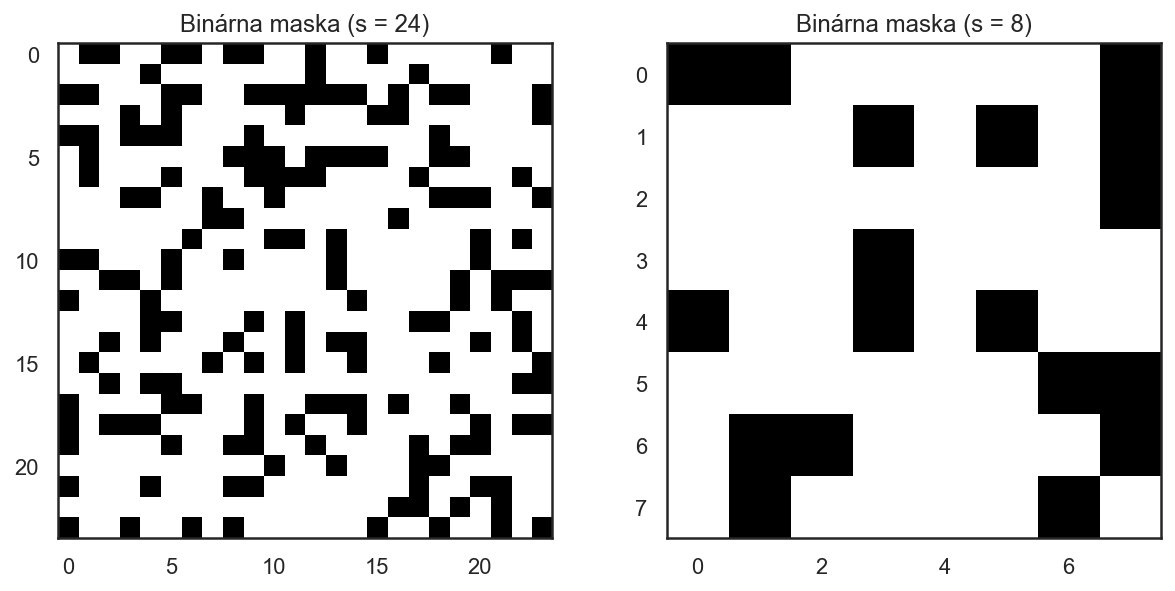
\includegraphics[width=13cm]{assets/images/binary_mask.png}
    \caption{Porovnanie dvoch binárnych masiek s rôznou veľkosťou (\textit{size}), čím väčšia veľkosť, tým je obrázok viac fragmentovaný.}
    \label{fig:binary_mask}
\end{figure}

\paragraph{Náhodné nastavenie pozície vyrezania, zväčšenie binárnej masky a orezenie na veľkosť obrázka}

Binárnu masku zväčšíme na veľkosť vstupného snímku plus menší offset (o veľkosti size). Následne zo zväčšenej masky na náhodnej pozícii vyrežeme masku o veľkosti vstupného snímku (Obr. \ref{fig:binary_mask_resized}). Táto maska určuje, ktoré miesta na snímku bude treba dokresliť - biele miesta, čiže jednotky. Tento krok v pôvodnej implementácii RISE nie je.

\begin{figure}[h!]
    \centering
    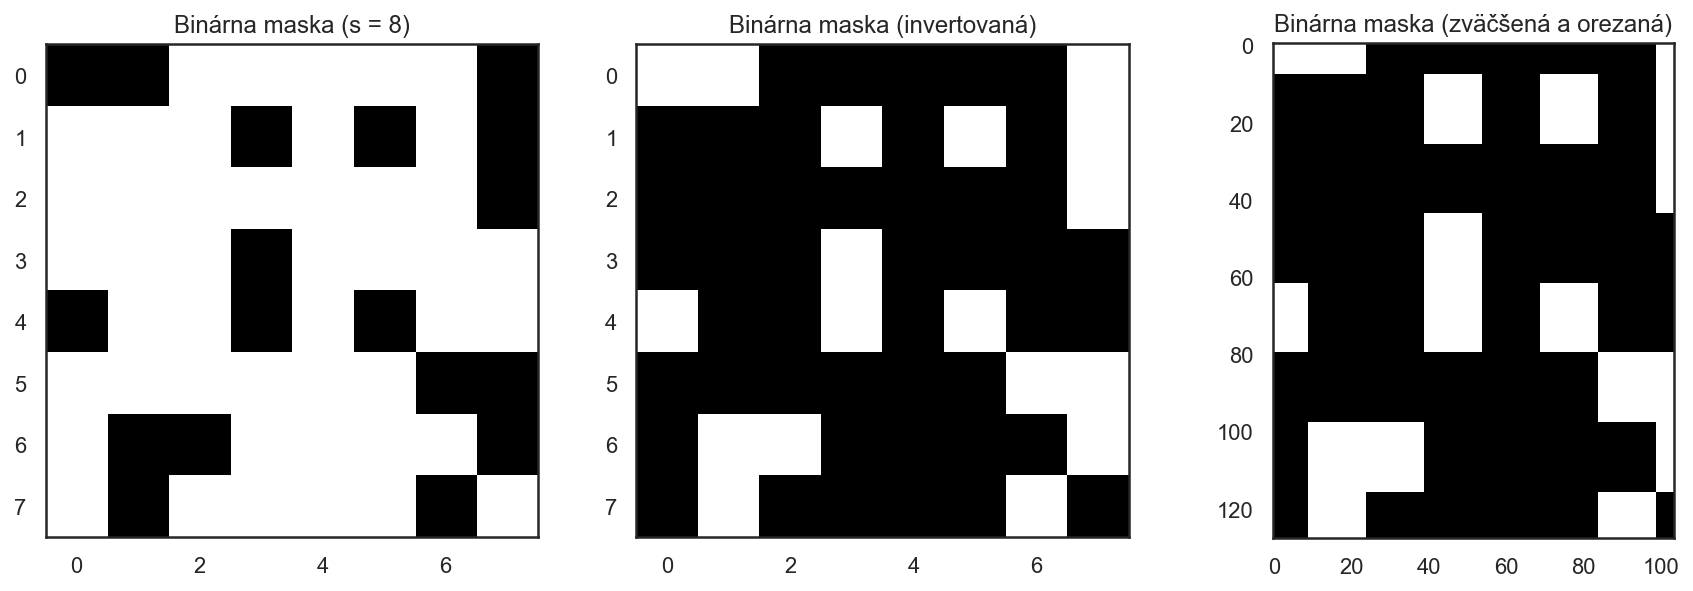
\includegraphics[width=13cm]{assets/images/binary_mask_resized.png}
    \caption{Vygenerovaná maska je zväčšená a orezaná na veľkosť vstupného snímku (ten je o veľkosti $[104, 128, 104]$ pričim na obrázkoch je vizualizovaná druhá a tretia dimenzia). Úplne vľavo je binárna maska o veľkosti $8$. V strede je invertovaná binárna maska (kvôli ďaľšiemu pracovanou s ňou) a vpravo je orezaná binárna maska o veľkosti vstupného snímku.}
    \label{fig:binary_mask_resized}
\end{figure}

\paragraph{Zväčšenie pomocou bilineárnej interpolácie a orezanie masky na veľkosť obrázka}

Tak ako v poôvodnej implementácii RISE, vytvoríme ''čiernu'' masku na zakrytie častí obrázku. Pôvodnú binárnu masku pomocou bilineárnej interpolácie (funkcia \textit{resize} z knižnice \textit{scikit-learn}) zväčšíme na veľkost vstupného snímku plus menší offset, následne vyrežeme na náhodnej pozicii masku o veľkosti vstupného snímku (táto náhodná pozícia je rovnaká ako pri orezávani binárnej masky bez interpolácie, preto je v BPMN diagrame v samostatnom kroku).

\begin{figure}[h!]
    \centering
    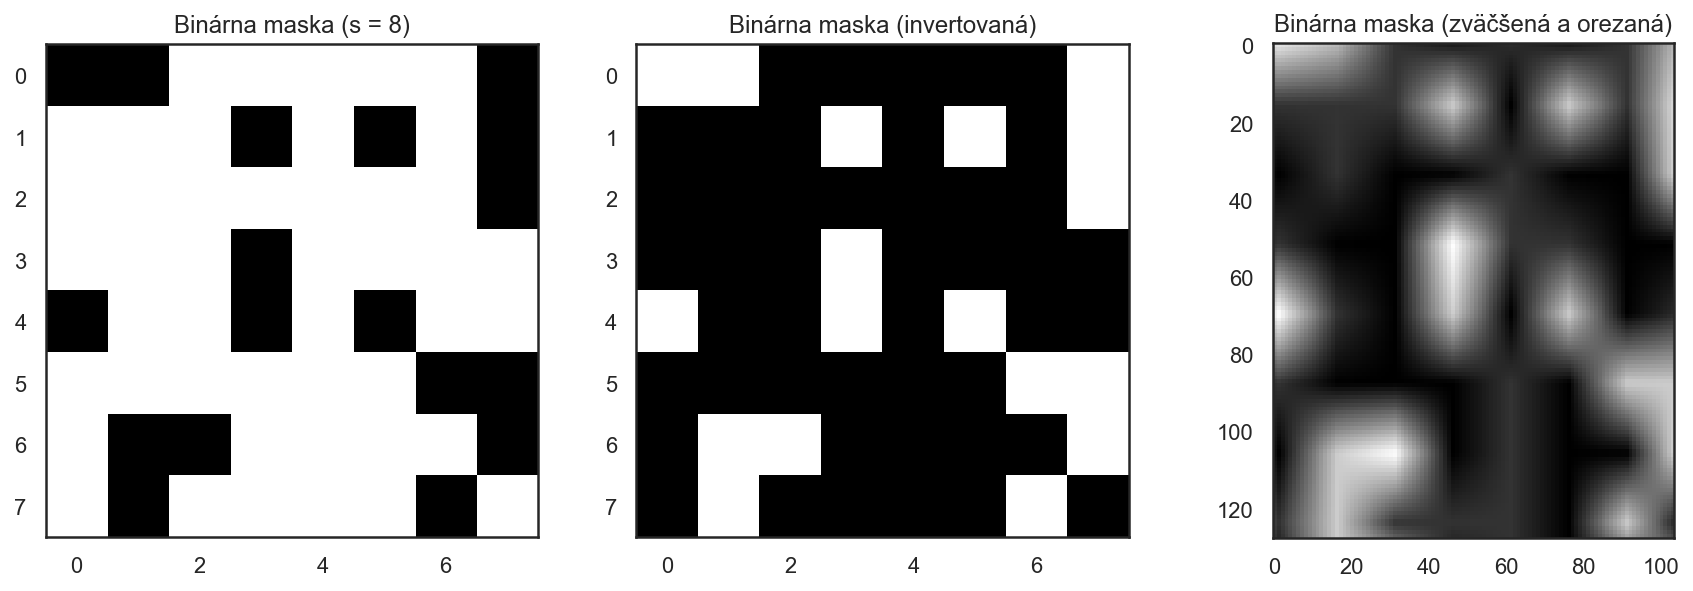
\includegraphics[width=13cm]{assets/images/interpolated_mask.png}
    \caption{Vygenerovaná maska je zväčšená pomocou bilineárnej interpolácie a orezaná na veľkosť vstupného snímku (ten je o veľkosti $[104, 128, 104]$ pričim na obrázkoch je vizualizovaná druhá a tretia dimenzia). Úplne vľavo je binárna maska o veľkosti $8$. V strede je invertovaná binárna maska (kvôli ďaľšiemu pracovanou s ňou) a vpravo je orezaná interpolovaná ''čierna'' maska o veľkosti vstupného snímku.}
    \label{fig:interpolated_mask}
\end{figure}

\paragraph{Prekrytie masky s obrázkom a dokreslenie zamaskovaných častí obrázka}

Keďže pracujeme nad trojrozmernými dátami, pokúsili sme sa použiť dokreslovanie obrázka v 3D. Na to sme sa pokúsili použiť funkciu \textit{inpaint} s knižnice \textit{scikit-image}, avšak dokreslenie jednej masky bolo veľmi časovo náročné (trvanie bolo až v minútach kde dokreslenie v 2D je v sekundách) a my ich potrebujeme generovať tisíce, preto sme trojrozmerného dokreslovania upustili.

Dokreslovanie dvojrozmerných snímkov z 3D snímku má avšak svoje nevýhody. Nech máme snímky o veľkosti $[z, y, x]$, pri 2D dokreslení musíme dokreslovať $z$ snímkov o veľkosti $[y, x]$ (alebo $y$ snímkov o veľkosti $[y, x]$, alebo $x$ snímkov o veľkosti $[y, z]$). Pri takomto dokreslovaní, dokreslenie z pohľadu $[y, x]$ vyzerajá byť správne, avšak z iného pohľadu, napr. $[z, x]$ sa javí byť dokreslenie nesprávne, najmä kvôli vzniknutým ostrím hranám (Obr. \ref{fig:inpaint_3x_2d}). Toto sme sa pokúsili obýsť tak, že dokreslujeme zo všetkých troch pohľadov a robíme priemer pre každý voxel zo všetkých troch dokreslení. Takto je výsledok o niečo lepší, tj. z každej strany je dokreslenie lepšie ako nesprávne dokreslenie z 2D ale o niečo horšie ako správne dokreslenie z 2D. Na označenie miest, ktoré treba dokresliť sme použili zväčšenú binárnu masku (Obr. \ref{fig:binary_mask_resized}). Dokreslenie vykonávame funkciou \textit{inpaint} z knižnice \textit{cv2 (Open CV)}. Používame dokreslovací algoritmus \textit{cv2.INPAINT\_TELEA}, keďže pomocou neho sme dosahovali vizuálne najlepšie výsledky. Funkcia \textit{cv2.inpaint} vyžaduje ako parameter \textit{inpaint\_radius} (Obr. \ref{fig:inpaint_radius}), čo je jedným z hyper parametrov našej metódy.

\begin{figure}[h!]
    \centering
    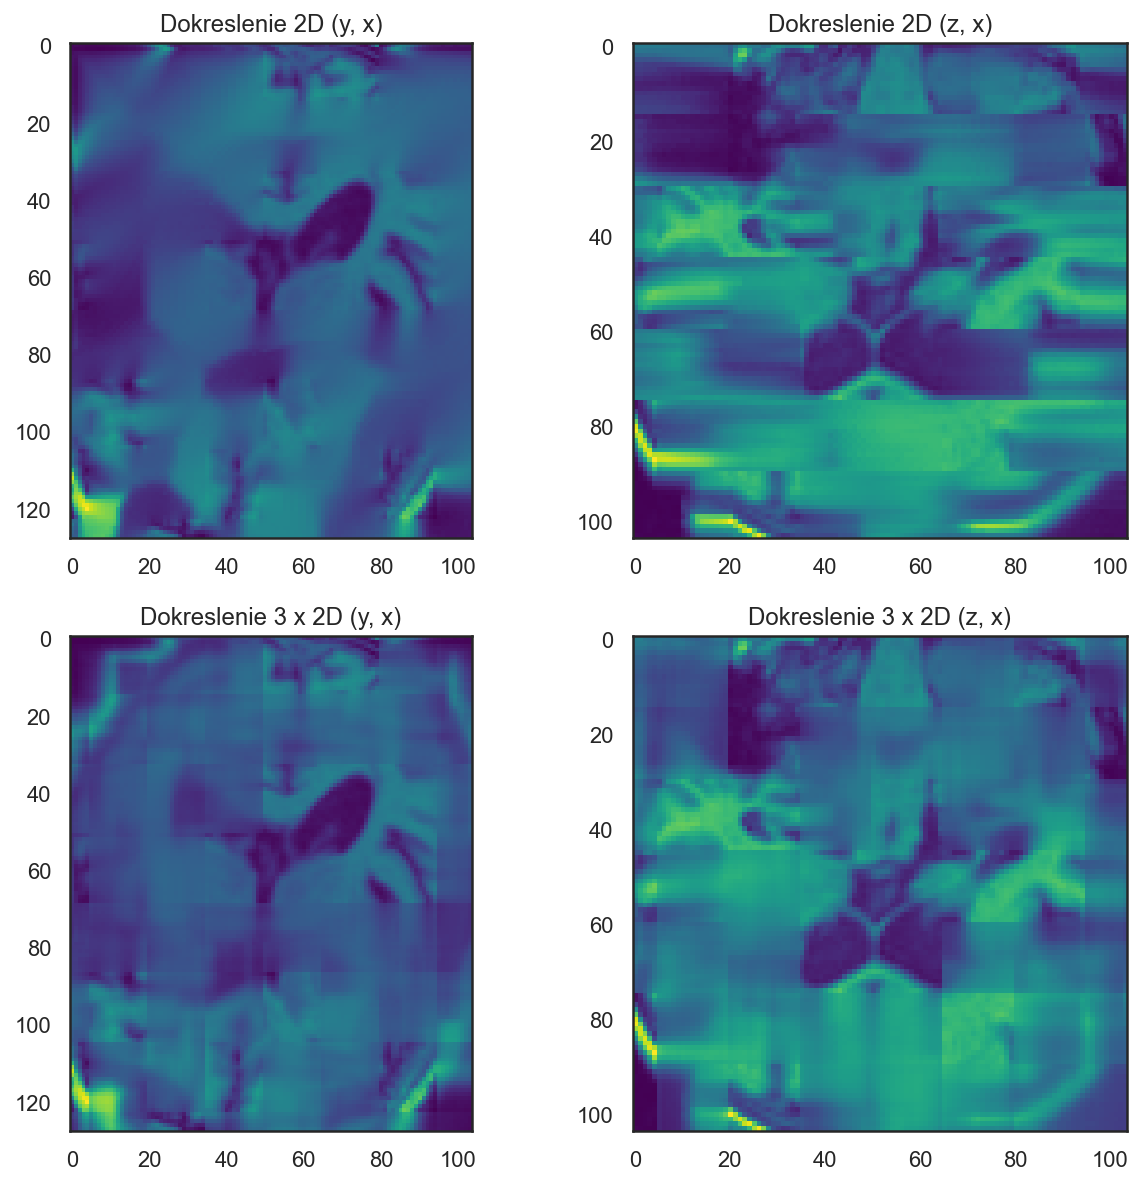
\includegraphics[width=13cm]{assets/images/inpaint_3x_2d.png}
    \caption{Porovnanie 2D dokreslenia (iba v jednej dimenzii) a spriemerovaného 3x 2D dokreslenia (v každej dimenzii). Použitie iba 2D dokreslenia je kvalitné iba v jednej dimenzii a v ostatných je deštruktívne - vytvára ostré hrany. Použitie 3x 2D dokreslenia a spriemerovanie pre každý voxel produkuje celkom dobré dokreslenia po všetkých dimenziách.}
    \label{fig:inpaint_3x_2d}
\end{figure}

Keďže sa pôvodná implementácia RISE prekrýva miesta tak, aby nevznikali ostré hrany medzi zakrytím miestom a pôvodným obrázkon, a teda vznikol plynulý prechod, aj pri dokreslení vytvárame plynulý prechod medzi dokreslením a pôvodným obrázkom (Obr. \ref{fig:inpaint_soft_corners}). Tento prechod je implementovaný nasledovne.
\begin{lstlisting}
    # binary_mask int[z, x, y] - upsized binary mask
    # image float[z, x, y] - original image
    # mask float[z, x, i] - upsizded and interpolated binary mask
    # inpaint_radius int
    inpainted = cv.inpaint(image, binary_mask, inpaint_radius, cv2.INPAINT_TELEA)
    inpainted_blend = image * mask + inpainted * (1 - mask)
\end{lstlisting}

\begin{figure}[h!]
    \centering
    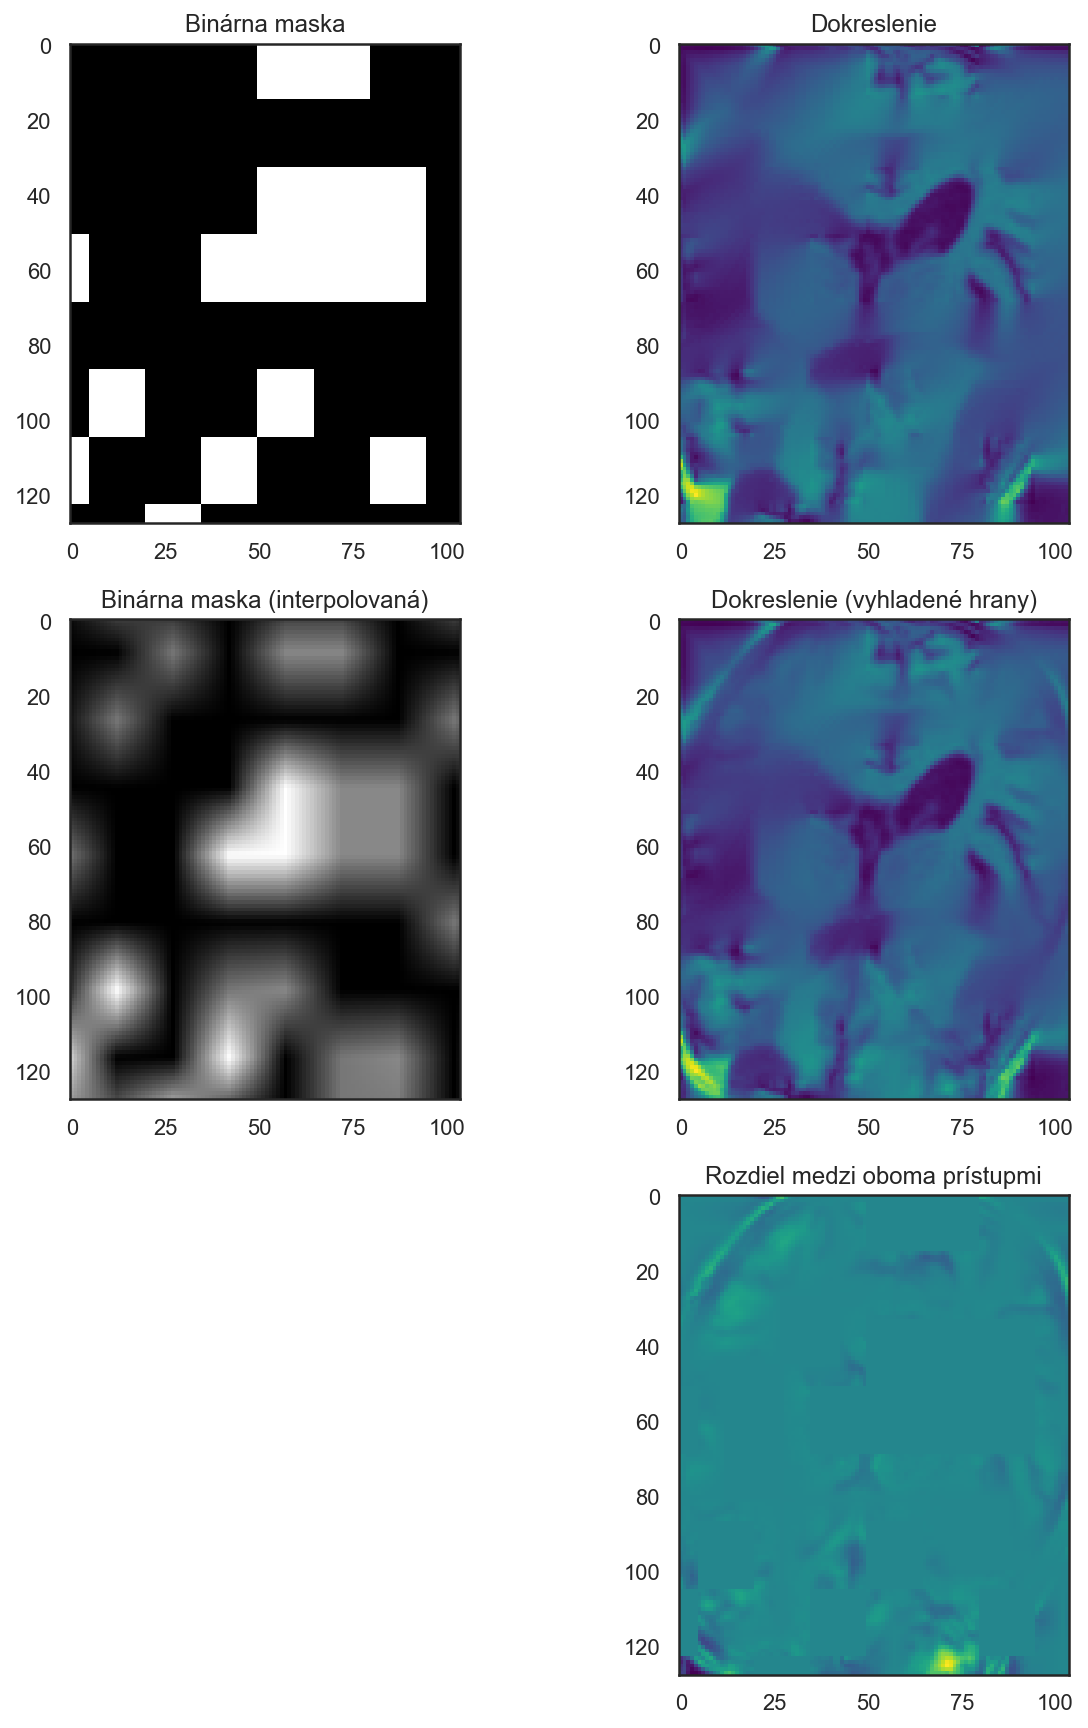
\includegraphics[width=10cm]{assets/images/inpaint_soft_corners.png}
    \caption{Príklad vyhladzovania hrán dokreslenia - splynutie dokreslenia s pôvodným snímkom (štvrtý snímok). Druhý snímok zobrazuje ostré hrany po dokreslení - bez splývania s obrázkom. Piaty snímok zobrazuje rozdiel medzi oboma prístupmi. Môžeme si všimnúť, že na obrázku sí viditeľné miesta, kde sa nachádza prechod na interpolovanej binárnej maske. O tieto miesta (informácie) je dokreslenie s vyhladenými hranami ''bohatšie''.}
    \label{fig:inpaint_soft_corners}
\end{figure}

\begin{figure}[h!]
    \centering
    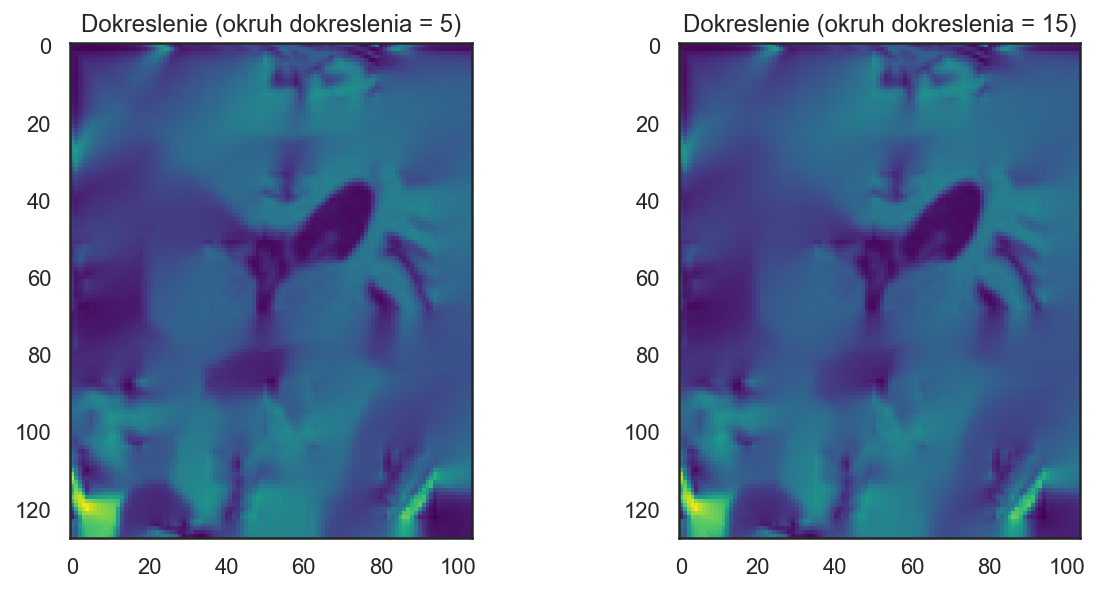
\includegraphics[width=13cm]{assets/images/inpaint_radius.png}
    \caption{Porovnanie okruhov dokreslenia (parameter \textit{inpaint\_radius}), rozdiel vo výsledku nie je veľmi viditelný, avšak s väčśím oruhom dokreslenia je generovanie rádovo pomalšie. (pri generovaní bolo vypnuté splynutie dokreslenia so snímkom aby bol rozdiel aspoň trochu viditeľný)}
    \label{fig:inpaint_radius}
\end{figure}

\paragraph{Prekrytie dokreslenej masky a čiernej masky s obrázkom}

Keďže prekrývam tri rôzne vrstvy - originálny snímok, čiernu masku a dokreslený snímok môžem tieto vrstvy skombinovať v rôznom pomere a tým vytvoriť nový obrázok.

Toto som implementoval zavedením parametrov $b1$ a $b2$ (skratka od slova prechod, angl. blend), ktoré hovoria o pomere medzi originálnym snímkom a dokresleným snímkom, a originálnym snímkom spojeným s dokreslením a čiernou maskou (Obr. \ref{fig:risei_layers}). Pri týchto parametroch platí, že $0 <= b1, b2 <= 1$. Takto zadefinované parametre mi umožňujú vytvoriť zakaskovaný snímok iba s čiernou maskou ($b1 = 0$, $b2 = 1$) či iba s dokreslením ($b1 = 1$, $b2 = 0$).

\begin{figure}[h!]
    \centering
    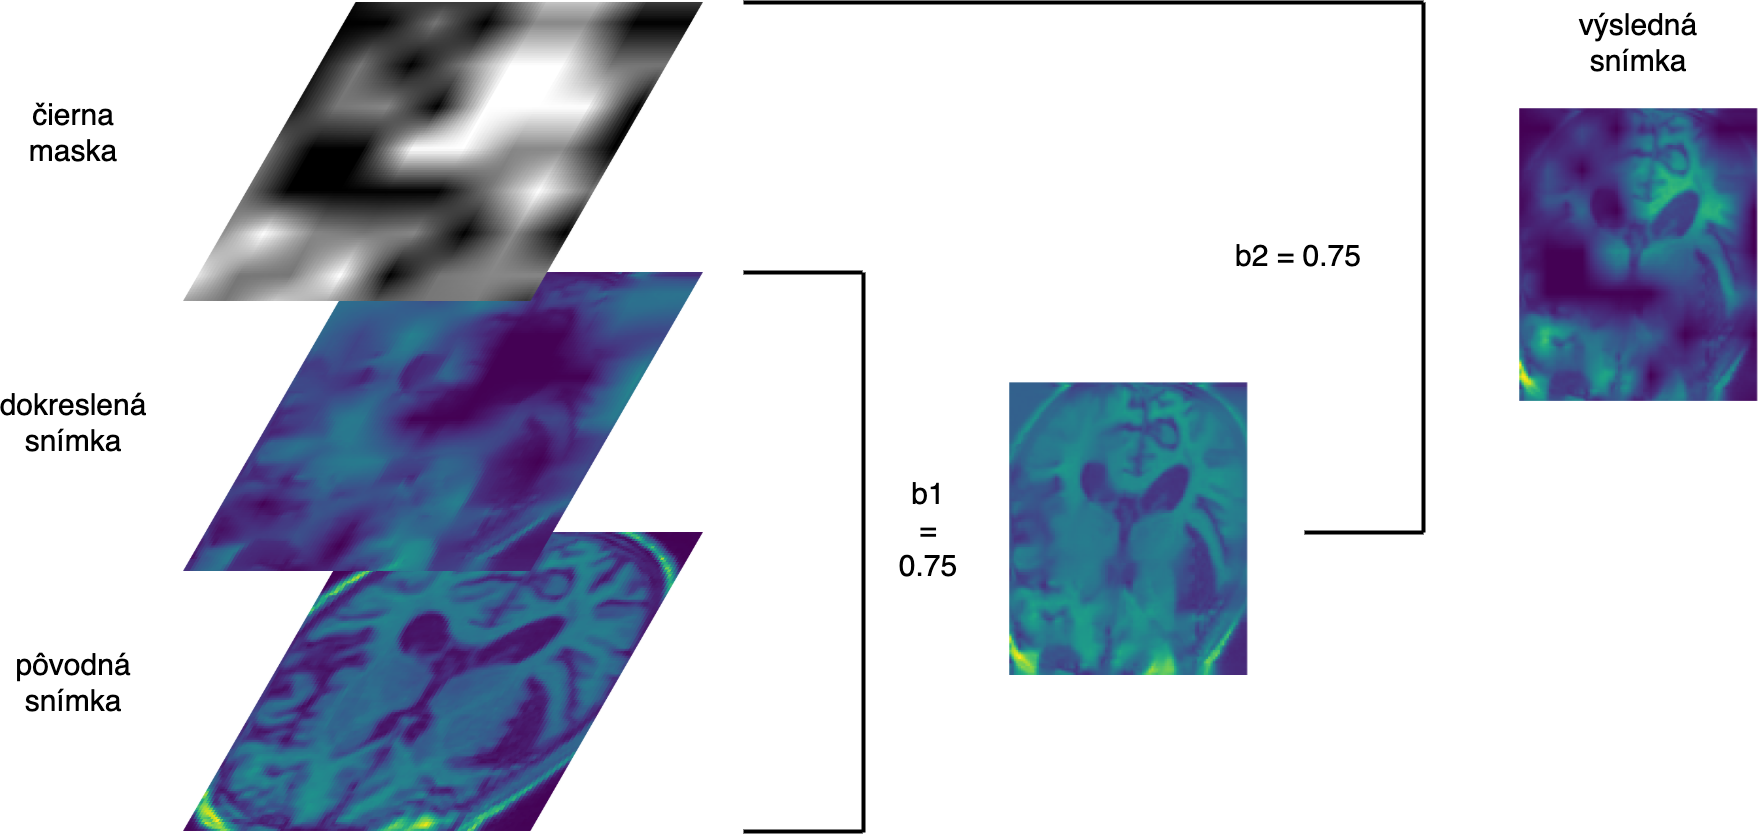
\includegraphics[width=13cm]{assets/images/risei_layers.png}
    \caption{Príklad, ako vyzerá spojenie originálneho snímku, dokresleného snímku a čiernej masky. V diagrame je zobrazený aj výsledok medzikroku spojenia dokresleného snímku a pôvodného snímku. Parametre boli nastavené na $b1 = 0.75$ a $b2 = 0.75$.}
    \label{fig:risei_layers}
\end{figure}

Názov ''čierna'' maska pochádza z pôvodnej implementácie RISE, kde sa obrázok prekrýval čiernou maskou. V našej implementácii neprekrývame farbou, ale hodnotou, tj. ''čierna'' je hodnota $0$ (minimum). Okrem použitia hodnoty $0$, môžeme použiť aj $1$, \textit{priemer} či \textit{medián} (toto je ďaľším hyper-parametrom našej metódy). Zjednodušená (a menej efektívna, v produkčej implementácii sa niektoré inštrukcie nevykonávajú keď \textit{b1} je 0 alebo \textit{b2} je 0) implementácia spojenia jednitlivých vrstiev vyzerá nasledovne.

\begin{lstlisting}
    # image float[z, x, y] - original image
    # inpainted_blend float[z, x, y] - inpainted image
    # mask float[z, x, i] - upsizded and interpolated binary mask
    # b1 float <0, 1>
    # b2 float <0, 1>
    # b2_value string - what value use in "black" mask (min/max/mean/median)

    # merge with inpainted image
    new_image = (1 - b1) * original_image + b1 * inpainted_blend

    value = 0 # black
    if b2_value == 'max':
        value = 1 # white
    elif b2_value == 'mean':
        value = np.mean(original_image)
    elif b2_value == 'median':
        value = np.median(original_image)
    # merge with "black" mask
    new_image = b2 * mask * new_image + (b2 * (1 - mask) * value)
\end{lstlisting}

Kompletný zoznam parametrov metódy RISEI sa nachádza v tabuľke \ref{tab:rise_params}.

\begin{table}[]
    \begin{tabular}{p{0.25\linewidth} | p{0.15\linewidth} | p{0.5\linewidth}}
        \hline
        Názov              & Dátový typ & Popis                                                               \\ \hline
        size              & int       & Veľkosť strany binárnej 3D matice.                                        \\
        probability       & float     & Pravdepodobnosť, že plocha nebude prekrytá maskou.                        \\
        b1                & float     & Miera prekrytia medzi originálnym snímkom a dokresleným snímkom.          \\
        b2                & float     & Miera prekrytia s ''čiernou'' maskou.                                     \\
        b2\_value         & string    & Hodnota ''čiernej'' masky, môže to byť minimum, maximum, medián, priemer. \\
        in\_paint\_radius & float     & Polomer dokreslenia algoritmom z knižnice OpenCV.                         \\ \hline
        \end{tabular}
    \caption{Zoznam parametrov metódy RISEI.}
    \label{tab:rise_params}
\end{table}

\subsection{Vytvorenie tepelných máp}

% TODO:

\section{Model na detekciu Alzheimerovej choroby na základe MRI snímkov}